\scanpage{11}
Carte trouée
\diagram{\begin{tikzcd}[ampersand replacement=\&,column sep=small]
(X\arrow[d]\supset K\arrow[dr])\&\&\text{tels que}\\
\text{surf. top.}\&\begin{gathered}\text{sous-variété fermée}\\\text{de dim 1}\end{gathered}\&
\end{tikzcd}}

\unsure{tte} comp. de $\operatorname{Déc}(X,K)$ est homéomorphe à un $D_n^*$

(disque troué \unsure{standart}, $1\leq n\leq+\infty$)

$\Pi_n$ pol. comb. \unsure{ép.} d'ordre $n$
\[
\uline{|\Pi_n|\times]0,1]}\supset|\Pi_n|\supset S_n
\qquad
\begin{gathered}\Pi_n:(S_n,A_n,R_n)\\S_n\subset|\Pi_n|\end{gathered}
\]
\[
D_n^*=|\Pi_n|\times]0,1]\setminus S_n
\]

\figure{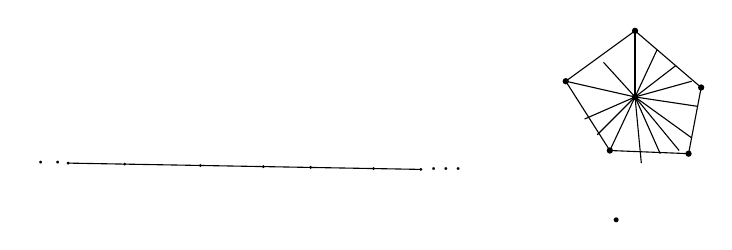
\begin{tikzpicture}[x=.8cm,y=.8cm]
\draw (9,3.1)--(10.05,2.2)--(9.85,1.15)--(8.6,1.2)--(7.9,2.3)--cycle;
\foreach \x/\y in {9/3.1,10.05/2.2,9.85/1.15,8.6/1.2,7.9/2.3,9/2.05}{\fill (\x,\y) circle(.05);}
\foreach \x/\y in {9/3.1,9.35/2.8,9.65/2.55,9.9/2.3,10/1.9,9.9/1.4,9.7/1.2,9.4/1.15,9.1/1.0,8.6/1.2,8.4/1.45,8.2/1.7,7.9/2.3,8.5/2.6}{\draw (9,2.05)--(\x,\y);}
\node at (-.3,1) {$\cdot\ \cdot$};
\draw (0,1)--(5.6,.9);
\foreach \x in {0,.9,2.1,3.1,3.85,4.85,5.6}{\fill (\x,{1-.1*\x/5.6}) circle(.025);}
\node at (6,.9) {$\ldots$};
\fill (8.7,.1) circle(.04);
\end{tikzpicture}}

\figure{\begin{tikzpicture}[x=.8cm,y=.8cm]
\draw[->] (3.4,6.2)--(1.3,5.55);
\draw[->] (2.55,5.75)--(2.2,6.35);
\draw[->] (3.8,6.2)..controls(4.5,5.95)and(5.3,6)..(5.9,5.65);
\draw[->] (4.55,5.85)--(4.7,6.3);
\draw[->,thick] (6.2,5.35)--(7.15,4.05);
\draw (7.1,4.25)..controls(7.4,3.9)and(7.5,3.6)..(7.45,3.5);
\draw (3.4,5.9)--(1.7,3);
\draw (5.15,4.9)--(5,4.4);\draw (4.9,4.2)--(3.65,2.1);
\draw (7.1,3.4)..controls(7,2.8)and(6.8,2.3)..(6.5,1.9);
\draw (7.6,3.3)..controls(7.85,2.3)and(7.5,1.8)..(7.65,1.2);
\node at (3.5,.8) {$E$};
\node at (1,.65) {$\uline{\sigma_0\ \sigma_1}\ \sigma_2$};
\draw (9.6,5.45) ellipse (1.02 and .94);
\draw (10.65,6.9)--(10.65,3.1);
\draw[thick] (9.6,5.45)--(10.65,5.4);
\draw (8.8,4.85)--(10.75,6.25);
\draw (8.8,4.85)--(8.91,5.03)--(8.96,4.86)--(9.03,5.14)--(9.09,4.98)--(9.16,5.22)--(9.22,5.07)--(9.29,5.31)--(9.35,5.18)--(9.48,5.4);
\foreach \x/\y in {9.45/6.38,8.65/5.75,8.8/4.85,9.82/4.51,10.63/5.16,10.65/5.4,10.42/6.0,9.6/5.45}{\fill (\x,\y) circle(.045);}
\draw[->,thick] (9.4,4.53)--(9,4.62);
\node at (11.65,5.7) {$\pm\frac1n$};
\draw (9.45,1.95) ellipse (1.15 and 1.1);
\draw[line width=2pt] (9.25,3.04) arc[start angle=100,end angle=38,x radius=1.15,y radius=1.1];
\draw[line width=2pt] (10.52,1.58)--(10.35,1.19);
\draw[line width=2pt] (10.05,1.02)..controls(9.9,.8)and(9.65,.81)..(9.4,.82);
\draw[line width=2pt] (8.31,2.25)--(8.31,1.55);
\draw[->,thick] (8.65,2.8)--(8.32,2.57);
\draw (8.3,2.52)--(8.45,2.32);\draw (8.19,2.2)--(8.43,2.22);
\draw[->] (9.4,1.4)..controls(10,1.6)and(10,1.9)..(9.9,2.2);
\draw[dashed] (12.65,1.48) circle(.25);
\draw[gray,densely dotted] (12.9,.65) circle(.3);
\draw (13.1,-.15) circle(.17);\draw[gray] (13.12,-.13) circle(.17);
\end{tikzpicture}}

\figure{\begin{tikzpicture}
\node[draw,inner sep=8pt] at (5,3.5) {$\operatorname{Déc}(\hat X,\unsure{\omega|W})$};
\node at (8.4,3.4) {$\tilde X-F$};
\draw (2.1,3.55)--(2.4,3.2)--(3.8,2.55)--(3.5,.9)--(2,{.2+1})--(1.65,2.65)--cycle;
\draw (2.1,3.55)--(1.85,4.1);\draw (2.1,3.55)--(2.4,3.95);
\draw (1.65,2.65)--(.6,2.75);\draw (1.65,2.65)--(1.55,3.3)--(2.1,3.55);
\draw (2.4,3.2)--(1.65,2.65);
\draw (3.8,2.55)--(4.5,3);\draw (3.5,.9)--(3.8,.5);\draw (2,1.2)--(1.7,.5);
\foreach \x/\y in {2.4/3.2,3.8/2.55,3.5/.9,2/1.2,1.65/2.65}{\fill (\x,\y) circle(.04);\draw (\x,\y) circle(.19);}
\draw (2.7,2.1) circle(.15);\fill (2.7,2.1) circle(.035);
\draw (5.3,2)--(5.8,2.45);\draw (5.3,2)--(5.25,2.45);\draw (5.3,2)--(4.95,2.2);\draw (5.3,2)--(4.9,1.65);\draw (5.3,2)--(5.4,1.65);\draw (5.3,2)--(5.85,1.95);
\end{tikzpicture}}

\mspage{10}
